\documentclass[11pt,a4paper]{article}

\usepackage{fontspec}
\usepackage[french]{babel}
\usepackage[margin=2.2cm]{geometry}
\usepackage{amsmath,amssymb}
\usepackage{graphicx}
\usepackage{booktabs}
\usepackage{array}
\usepackage{xcolor}
\usepackage[most]{tcolorbox}
\usepackage{enumitem}
\usepackage{hyperref}

\hypersetup{colorlinks=true, linkcolor=blue!50!black, urlcolor=blue!50!black}
\setlist{itemsep=2pt, topsep=4pt}

\newtcolorbox{aretenir}{colback=blue!4, colframe=blue!50!black, fonttitle=\bfseries,
  title=À retenir, sharp corners, boxrule=0.6pt}
\newtcolorbox{alimite}{colback=orange!6, colframe=orange!70!black, fonttitle=\bfseries,
  title=Attention / limite, sharp corners, boxrule=0.6pt}
\newtcolorbox{adire}{colback=green!5, colframe=green!40!black, fonttitle=\bfseries,
  title=À dire au professeur, sharp corners, boxrule=0.6pt}

\title{\textbf{Nappe de volatilité implicite du CAC 40}\\[4pt]
\large Fiche de synthèse : ce qu'on a fait et ce qu'il faut retenir}
\author{Projet de fin d'études}
\date{Données relevées le 26 novembre 2026}

\begin{document}
\maketitle

\begin{aretenir}
\begin{enumerate}[leftmargin=*]
  \item La \textbf{volatilité implicite} est le $\sigma$ qui, mis dans la formule de Black-76,
        redonne le prix observé sur le marché.
  \item Elle \textbf{dépend du strike et de la maturité} (smile / skew, nappe en 3D) :
        c'est la preuve que l'hypothèse de vol constante de Black-Scholes est fausse.
  \item Sur le CAC 40, les \textbf{puts loin sous le forward ont une vol plus élevée} :
        le marché a peur des krachs et paie pour s'en protéger.
  \item La vol implicite est \textbf{en général au-dessus de la vol historique} :
        c'est la \textbf{prime de volatilité}.
\end{enumerate}
\end{aretenir}

\tableofcontents

% ==============================================================================
\section{Objectif de l'exercice}

Dans la formule de Black-Scholes, tous les paramètres sont observables (spot, strike,
maturité, taux, dividendes) \textbf{sauf la volatilité $\sigma$}. On renverse donc le
raisonnement : au lieu de partir de $\sigma$ pour calculer un prix, on part du \textbf{prix
de marché} pour retrouver le $\sigma$ que le marché « utilise ». C'est la volatilité implicite.

Le travail consistait à :
\begin{enumerate}[leftmargin=*]
  \item construire la \textbf{nappe de volatilité implicite} du CAC 40 à partir de prix réels ;
  \item la \textbf{comparer à la volatilité historique} de l'indice.
\end{enumerate}

% ==============================================================================
\section{Les données}

\begin{itemize}[leftmargin=*]
  \item \textbf{200 warrants SG sur le CAC 40} (100 calls, 100 puts), 6 échéances de
        décembre 2026 à juin 2027. Spot du CAC 40 : $S \approx 8139$ points.
  \item \textbf{Parité} : un warrant 200:1 vaut $1/200$ d'option. Prix d'une option sur l'indice :
        \[ \text{prix option} = \text{prix warrant} \times \text{parité}. \]
  \item \textbf{Prix milieu} : $\dfrac{\text{achat} + \text{vente}}{2}$.
  \item \textbf{Historique} : cours de clôture du CAC 40 sur 2 ans (Yahoo Finance, \texttt{\^{}FCHI}).
\end{itemize}

\textbf{Nettoyage :}
\begin{itemize}[leftmargin=*]
  \item on retire les warrants à 0,01--0,02~€ : leur prix est trop arrondi pour donner une vol fiable ;
  \item on retire les échéances à moins de 7 jours ;
  \item on garde seulement les options \textbf{hors de la monnaie} (OTM) : puts avec $K < F$, calls avec $K > F$.
\end{itemize}

\begin{aretenir}
\textbf{Pourquoi seulement les options hors de la monnaie ?} Une option dans la monnaie vaut surtout
sa valeur intrinsèque (ce qu'elle rapporterait si on l'exerçait tout de suite) : son prix contient peu
d'information sur la volatilité. Une option hors de la monnaie n'a \emph{que} de la valeur temps,
donc son prix dépend presque entièrement de $\sigma$.
\end{aretenir}

% ==============================================================================
\section{Le forward par la parité call-put}

Le \textbf{forward} $F$ est le prix, fixé aujourd'hui, auquel on achèterait le CAC 40 à la date $T$.
Il tient compte des dividendes versés d'ici là.

Pour un call et un put de même strike $K$ et même maturité $T$ :
\[
  C - P = e^{-rT}\,(F - K)
  \qquad\Longrightarrow\qquad
  F = K + e^{rT}\,(C - P).
\]
On applique cette formule aux strikes cotés à la fois en call et en put, et on fait la moyenne sur
les 3 plus proches du spot. Taux sans risque : $r = 2{,}5\,\%$.

\begin{center}
\begin{tabular}{lrl}
\toprule
Échéance & Forward $F$ & Méthode \\
\midrule
18/12/2026 & 8145 & parité call-put \\
15/01/2027 & 8160 & parité call-put \\
19/02/2027 & 8180 & parité call-put \\
19/03/2027 & 8204 & parité call-put \\
16/04/2027 & 8129 & secours : $S\,e^{(r-q)T}$, $q = 2{,}8\,\%$ \\
18/06/2027 & 8125 & secours : $S\,e^{(r-q)T}$, $q = 2{,}8\,\%$ \\
\bottomrule
\end{tabular}
\end{center}

\begin{alimite}
En avril et juin, aucun strike n'est coté à la fois en call et en put : on suppose un dividende
constant de 2,8\,\% par an. Or les dividendes du CAC 40 sont versés surtout en mai--juin :
ces deux forwards sont donc approximatifs.
\end{alimite}

% ==============================================================================
\section{Le modèle : Black-76}

Black-76 est la formule de Black-Scholes écrite avec le \textbf{forward} $F$ au lieu du spot $S$ :
\[
  C = e^{-rT}\big[F\,N(d_1) - K\,N(d_2)\big], \qquad
  P = e^{-rT}\big[K\,N(-d_2) - F\,N(-d_1)\big],
\]
\[
  d_1 = \frac{\ln(F/K) + \tfrac12 \sigma^2 T}{\sigma\sqrt{T}}, \qquad d_2 = d_1 - \sigma\sqrt{T}.
\]

\begin{aretenir}
\textbf{Black-76 et Black-Scholes avec dividende sont équivalents} : si on remplace
$F = S\,e^{(r-q)T}$ dans Black-76, on retombe exactement sur Black-Scholes avec un taux de
dividende $q$. Ils donnent le même prix et la même vol implicite.

\textbf{Pourquoi choisir Black-76 ?} Le forward contient déjà les dividendes. En le lisant sur
le marché (parité call-put), on évite de supposer un taux de dividende. C'est la méthode
standard pour les options sur indice.
\end{aretenir}

% ==============================================================================
\section{Le calcul de la volatilité implicite}

On cherche $\sigma$ tel que
\[
  \text{Black76}(F, K, T, r, \sigma) = \text{prix observé}.
\]
Il n'existe pas de formule pour isoler $\sigma$. On le trouve \textbf{numériquement} avec la
méthode de Brent (\texttt{brentq}), qui cherche le zéro de
$f(\sigma) = \text{Black76}(\sigma) - \text{prix}$ entre $1\,\%$ et $200\,\%$.

Il y a toujours une seule solution, car le prix d'une option \textbf{augmente toujours quand
$\sigma$ augmente} (le vega est positif).

% ==============================================================================
\section{Le smile et la nappe de volatilité}

\begin{figure}[h!]
  \centering
  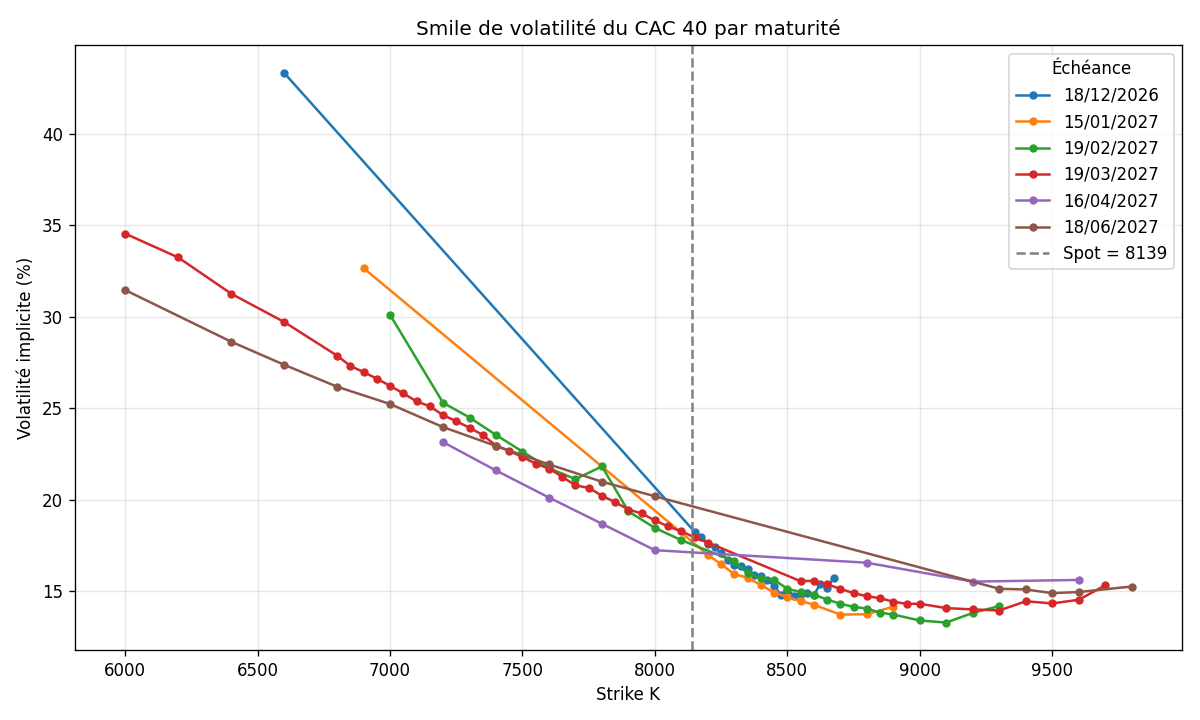
\includegraphics[width=0.85\textwidth]{figures/1_smiles.png}
  \caption{Smile de volatilité implicite par maturité.}
\end{figure}

\textbf{Constat :}
\begin{itemize}[leftmargin=*]
  \item calls au-dessus du forward : vol $\approx 14$--$15\,\%$ ;
  \item à la monnaie : vol $\approx 17$--$18\,\%$ ;
  \item puts loin sous le forward : vol de $25$ à plus de $40\,\%$.
\end{itemize}

\begin{aretenir}
\begin{itemize}[leftmargin=*]
  \item Si Black-Scholes était vrai, on trouverait \textbf{la même vol pour tous les strikes}
        (une droite horizontale). Ce n'est pas le cas.
  \item Sur un indice actions, la courbe penche vers la gauche : on parle de \textbf{skew}.
  \item \textbf{Raison :} les investisseurs craignent les krachs bien plus que les fortes hausses.
        Ils achètent beaucoup de puts pour se protéger, ce qui fait monter leur prix, donc leur vol.
  \item Le marché anticipe des baisses brutales plus probables que ce que prévoit la loi normale
        (« queues épaisses »).
\end{itemize}
\end{aretenir}

\begin{figure}[h!]
  \centering
  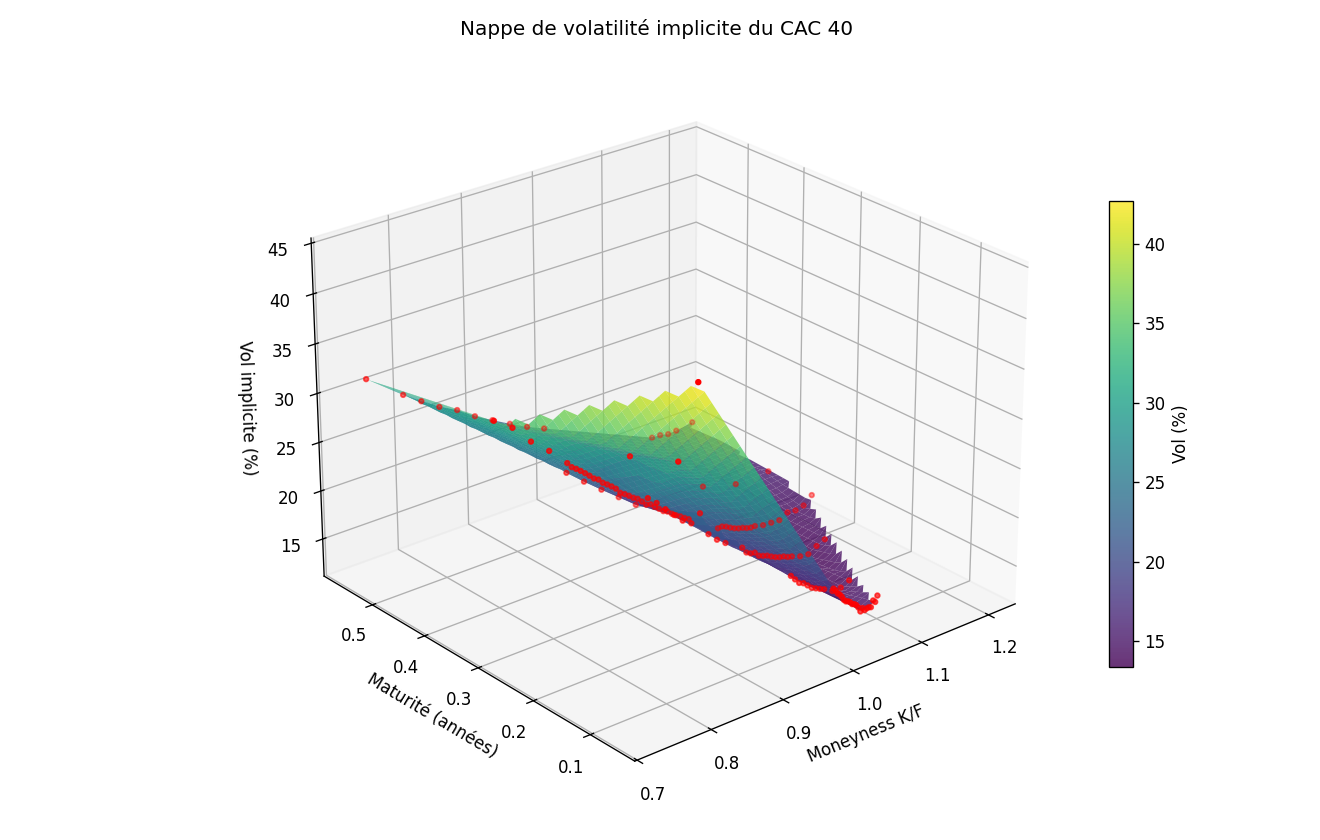
\includegraphics[width=0.85\textwidth]{figures/2_nappe_3d.png}
  \caption{Nappe de volatilité implicite : vol en fonction de la moneyness $K/F$ et de la maturité.}
\end{figure}

En ajoutant la maturité, on obtient la \textbf{nappe} (ou surface) de volatilité :
$\sigma = f(K, T)$.
\begin{itemize}[leftmargin=*]
  \item Le skew est \textbf{plus marqué sur les échéances courtes} et s'aplatit avec la maturité.
  \item \textbf{À quoi ça sert :} pour donner le prix d'une option non cotée (autre strike, autre date),
        une banque lit la vol sur la nappe et la met dans son modèle. Un trader n'utilise pas
        une vol unique, mais toute la nappe.
\end{itemize}

% ==============================================================================
\section{Volatilité historique contre volatilité implicite}

\subsection{Définition de la vol historique}

\[
  R_t = \ln\!\left(\frac{P_t}{P_{t-1}}\right), \qquad
  \sigma_{\text{hist}} = \text{écart-type}(R_t) \times \sqrt{252}.
\]

\begin{aretenir}
\textbf{Pourquoi $\sqrt{252}$ ?} Il y a environ 252 jours de bourse par an. La variance augmente
proportionnellement au temps, donc la volatilité augmente comme la \textbf{racine} du temps :
on passe d'une vol journalière à une vol annuelle en multipliant par $\sqrt{252}$.
\end{aretenir}

\begin{center}
\begin{tabular}{>{\raggedright}p{3.2cm}p{5.4cm}p{5.4cm}}
\toprule
 & \textbf{Vol historique} & \textbf{Vol implicite} \\
\midrule
Ce que c'est & Ce que le CAC \textbf{a bougé} & Ce que le marché \textbf{anticipe} \\
Calcul & Écart-type des rendements passés $\times\sqrt{252}$ & Inversion de Black-76 sur les prix \\
Orientation & Passé & Futur (+ prime de risque) \\
Dépend du strike ? & Non : un seul chiffre & Oui : smile / skew \\
\bottomrule
\end{tabular}
\end{center}

\subsection{Résultats}

\begin{figure}[h!]
  \centering
  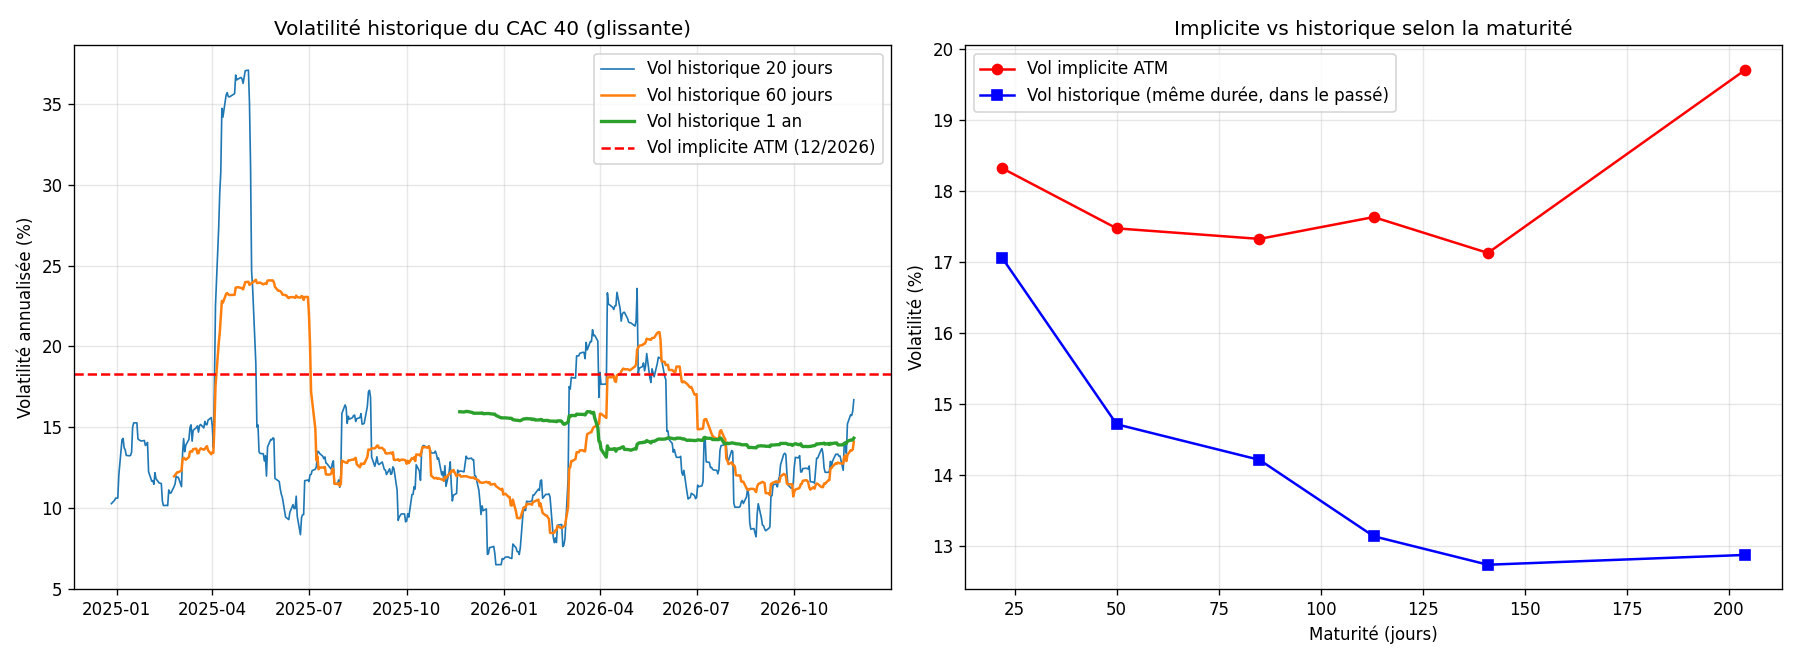
\includegraphics[width=\textwidth]{figures/3_vol_historique_vs_implicite.png}
  \caption{À gauche : vol historique glissante (20 jours, 60 jours, 1 an). À droite : vol implicite
  à la monnaie et vol historique sur une durée égale à la maturité.}
\end{figure}

\begin{center}
\begin{tabular}{lrrrr}
\toprule
Échéance & Jours & Vol implicite ATM & Vol historique & Écart \\
\midrule
18/12/2026 & 22  & 18,3\,\% & 17,1\,\% & $+1{,}2$ \\
15/01/2027 & 50  & 17,5\,\% & 14,7\,\% & $+2{,}7$ \\
19/02/2027 & 85  & 17,3\,\% & 14,2\,\% & $+3{,}1$ \\
19/03/2027 & 113 & 17,6\,\% & 13,1\,\% & $+4{,}5$ \\
16/04/2027 & 141 & 17,1\,\% & 12,7\,\% & $+4{,}4$ \\
18/06/2027 & 204 & 19,7\,\% & 12,9\,\% & $+6{,}8$ \\
\bottomrule
\end{tabular}
\end{center}

\begin{aretenir}
\begin{itemize}[leftmargin=*]
  \item La vol implicite est \textbf{toujours au-dessus} de la vol historique, de $+1$ à $+7$ points.
  \item C'est la \textbf{prime de volatilité} : les vendeurs d'options prennent un risque de krach
        et se font payer pour ça. Les acheteurs paient plus que le « juste prix statistique »
        pour être protégés, comme une assurance qui coûte en moyenne plus que les sinistres.
  \item La vol historique \textbf{varie beaucoup dans le temps} : plus de $35\,\%$ en avril 2025
        (période de forte baisse), $12$--$14\,\%$ ces dernières semaines. La volatilité n'est donc
        pas constante, ce qui contredit encore Black-Scholes.
\end{itemize}
\end{aretenir}

\begin{alimite}
Le chiffre de juin ($19{,}7\,\%$) est probablement surestimé : la vol ATM y est interpolée entre un put
à 8000 et un call à 9300, très éloignés, et le forward repose sur un dividende supposé.
\end{alimite}

% ==============================================================================
\section{Peut-on passer de l'une à l'autre ?}

\subsection{Retrouver la vol historique à partir de la vol implicite ? Non}

Ce sont deux grandeurs différentes :
\[
  \sigma_{\text{implicite}} \approx \text{vol future attendue} + \text{prime de risque}.
\]
La vol implicite ne contient aucune information sur le passé. Au mieux, c'est une
\textbf{prévision de la vol future}, et cette prévision est \textbf{trop haute en moyenne}
à cause de la prime.

On peut en revanche \textbf{comparer} :
\begin{itemize}[leftmargin=*]
  \item la vol implicite d'aujourd'hui à la vol historique passée (ce qui a été fait) ;
  \item ou, plus rigoureux, la vol implicite d'aujourd'hui à la vol \textbf{réalisée jusqu'à l'échéance}.
        Ça ne peut se vérifier qu'après coup.
\end{itemize}

\subsection{Retrouver le prix du warrant ?}

\textbf{Avec la vol implicite : oui, exactement.} C'est vrai par construction, puisque la vol implicite
a été calculée pour redonner ce prix. On calcule Black-76 avec la vol implicite, on divise par la parité,
et on retombe sur le prix de marché. C'est un bon \textbf{test de vérification du code}.

\textbf{Avec la vol historique : on obtient un prix « théorique » trop bas.}
Exemple pour l'échéance de mars 2027, avec une vol historique de $13{,}1\,\%$ :

\begin{center}
\begin{tabular}{lrrrr}
\toprule
Warrant & Prix marché & Vol implicite & Prix avec vol historique & Écart \\
\midrule
Put 7000  & 0,385\,€ & 26,2\,\% & 0,015\,€ & $-96\,\%$ \\
Put 7600  & 0,755\,€ & 21,7\,\% & 0,219\,€ & $-71\,\%$ \\
Put 8000  & 1,225\,€ & 18,9\,\% & 0,736\,€ & $-40\,\%$ \\
Call 8600 & 0,665\,€ & 15,6\,\% & 0,477\,€ & $-28\,\%$ \\
Call 9000 & 0,205\,€ & 14,3\,\% & 0,152\,€ & $-26\,\%$ \\
\bottomrule
\end{tabular}
\end{center}

\begin{aretenir}
\begin{itemize}[leftmargin=*]
  \item \textbf{Tous les warrants sont plus chers sur le marché} que leur prix avec la vol historique :
        c'est la prime de volatilité, exprimée en euros.
  \item \textbf{L'écart est énorme sur les puts loin sous le forward} (jusqu'à $-96\,\%$). Avec une vol
        historique unique, une baisse de $15\,\%$ en 4 mois paraît presque impossible, donc le put ne vaut
        presque rien. Le marché prend ce risque très au sérieux. \textbf{C'est le skew vu en euros.}
  \item \textbf{Conclusion :} on ne peut pas pricer correctement avec la vol historique. Les banques
        pricent avec la \textbf{nappe de vol implicite}.
\end{itemize}
\end{aretenir}

% ==============================================================================
\section{Limites du travail}

\begin{enumerate}[leftmargin=*]
  \item \textbf{Warrants et non options cotées} : les prix incluent la marge de Société Générale.
        On mesure la vol telle que SG la cote, proche du marché mais pas identique.
  \item \textbf{Données incomplètes} : l'export SG est limité à 100 lignes par fichier, donc il y a
        très peu de puts sur décembre et janvier.
  \item \textbf{Dividende supposé} pour avril et juin (pas de parité call-put possible).
  \item \textbf{Nappe sans modèle} : les points sont simplement reliés par interpolation linéaire.
        En pratique, on ajuste un modèle paramétrique (par exemple \textbf{SVI}) pour obtenir une
        surface lisse et sans arbitrage.
\end{enumerate}

% ==============================================================================
\section{Questions possibles du professeur}

\begin{description}[leftmargin=0.5cm, style=nextline]
  \item[Pourquoi Black-76 et pas Black-Scholes ?]
    Les deux sont équivalents si $F = S\,e^{(r-q)T}$. Black-76 évite de supposer le dividende,
    puisqu'on lit $F$ directement sur le marché.
  \item[Pourquoi seulement les options hors de la monnaie ?]
    Une option dans la monnaie vaut surtout sa valeur intrinsèque, donc son prix contient peu
    d'information sur la vol.
  \item[Pourquoi $\sqrt{252}$ ?]
    Environ 252 jours de bourse par an ; la variance croît proportionnellement au temps, donc la vol
    croît comme la racine du temps.
  \item[Pourquoi la vol implicite est-elle plus haute que l'historique ?]
    Prime de risque : les vendeurs d'options se font rémunérer pour le risque de krach.
  \item[Pourquoi les puts ont-ils une vol plus élevée ?]
    Demande de protection contre les baisses et peur des krachs : c'est le skew.
  \item[Peut-on pricer avec la vol historique ?]
    On obtient un prix trop bas, surtout pour les puts loin sous le forward. On price avec la nappe implicite.
\end{description}

% ==============================================================================
\section{Conclusion}

\begin{adire}
« On a construit la nappe de volatilité implicite du CAC 40 à partir de 200 warrants SG.
On a calculé le forward par la parité call-put, puis inversé la formule de Black-76 pour obtenir
la vol implicite de chaque option. La vol n'est pas constante : elle dépend du strike et de la
maturité, avec un skew marqué côté puts, ce qui montre les limites de Black-Scholes.
En la comparant à la vol historique, on constate qu'elle est toujours plus élevée, de 1 à 7 points :
c'est la prime de risque que le marché paie pour se protéger contre les baisses. Avec la vol
implicite, on retrouve exactement le prix des warrants ; avec la vol historique, on les sous-évalue
fortement, surtout les puts loin sous le forward. »
\end{adire}

\end{document}
